\chapter{Peierls-Hubbard model}
\label{chap:model}

As mentioned in section \ref{sec:scope}, treatments based in the adiabatic and antiadiabatic approximations are unable to describe properly the correlated electron-lattice motion in cuprate's Cu-O bonds.
An alternative to overcome this limitation is an exact treatment of a reduced system.
In this thesis we focus on the O(4)-Cu(1)-O(4) cluster in YBa$_2$Cu$_3$O$_7$.
We approximate this local environment as a three site cluster with two holes. 
Such approximation is justified as the Cu(1)-O(4) bond length (1.83 \AA) is far shorter than the Cu(2)-O(4) bond length ($\sim 2.41$ \AA) (see figure \ref{fig:YBCO_structure}), making charge transfer outside the cluster a much slower process than the charge dynamics inside the cluster. 
Although we cannot directly identify the three site cluster proposed in this model with a particular structure of the CuO plane, the general approach of charge transfer between hole rich regions and hole poor regions in the plane coupled to the lattice degrees of freedom is still valid, hence the general conclusions we draw from this model applicable to describe the structure of the CuO plane.

This thesis is based in a thorough analysis of that model hamiltonian so we devote this chapter to a detailed description of its components.
In section \ref{sec:hamiltonian-and-basis} we describe the hamitlonian and the basis used. 
Section \ref{sec:isotopic-model} reviews a method of incorporating isotopic substitutions in this model and defines \textit{isotopic shifts} in this context.
In section \ref{sec:lattice-distortions} we discuss a method of calculating real-space lattice distortions.
Next, in section \ref{sec:electronic-projection}, we describe a projection into definite electronic occupation states.
Section \ref{sec:model-parameters} reviews some literature suggesting possible choices of parameters and lists the parameters used in this work.
We review in section \ref{sec:classification} a method for identifying and classifiying the different excitations in this model.
Finally, section \ref{sec:comp_details} gives some computational details about our calculations.

\section{Hamiltonian and basis set}
\label{sec:hamiltonian-and-basis}

To describe two holes in the O(4)-Cu(1)-O(4) cluster with an electron-lattice (phonon) correlated movement we use a hamiltonian consisting of three parts:

\begin{equation}
  \label{eq:full-hamiltonian}
  H = H_{el} + H_{ph} + H_{el-ph}
\end{equation}

\noindent corresponding to the electronic contribution, the phonon energies and the electron-phonon (lattice) coupling, respectively \cite{Salkola1994}. 
The electron-phonon coupling term deviates this model from the Born-Oppenheimer (adiabatic) approximation and prevents the separation of hamiltionan eigenstates, $\Psi$, as products of purely electronic and phononic parts, $\Psi=\psi_{el}\psi_{ph}$, unless $H_{el-ph}=0$.
Nonetheless, as it will be discussed in section \ref{sec:classification}, even for coupling values greater than zero the hamiltonian eigenstates can be interpreted as mainly \textit{electronic} or \textit{phononic} in nature.

The electronic part is modeled as a single band Hubbard model for three sites with two holes in it. 
We only consider the two holes as having opposite spin because the energies of states with two charges with the same spin are much greater.
Explicitly, $H_{el}$ is written as

\begin{equation}
  \label{eq:electronic-part}
  H_{el} = \sum_{\sigma,i=1}^3 E_i n_{\sigma i} 
        + U\sum_{i=1}^3 n_{i\downarrow}n_{i\uparrow} 
        + t\sum_{\sigma} \left(c_{1\sigma}^\dagger c_{2\sigma} + c_{2\sigma}^\dagger c_{3\sigma} + H.c. \right)
\end{equation}

\noindent where we denoted $n_{i\sigma}=c_{i\sigma}^\dagger c_{i\sigma}$ as the hole-number operator with $c_{i\sigma}^\dagger$ creating a hole with spin $\sigma = \uparrow, \downarrow$ and $c_{i\sigma}$ destroying it; the site index $i=1,2,3$ indicates the two oxygen sites [O(4)] when  $i=1,3$ and the only copper site [Cu(1)] when $i=2$. 
The site energies are parametrized with $E_1=E_3=-E_2 \equiv E_0$. 
$U$ is the on-site Coulomb interaction and $t$ is the hopping energy between two adjacent sites. 

For the lattice  part of the Hamiltonian, $H_{ph}$, we consider both symmetric (Raman) and antisymmetric (infrared) modes described by boson operators $b_R$ and $b_{ir}$ and bare frequencies $\omega_R$ and $\omega_{ir}$ respectively\footnote{Unlike previous publications, here we include the \textit{zero-point energy} for both phonon modes. 
For most cases this is not needed since the excitation's energies are calculated relative to the ground state but, in chapter \ref{chap:ground} we study the ground state energy itself where this contribution is important},

\begin{equation}
 \label{eq:phonon-part}
 H_{ph} = \hbar \omega_{ir}\left(b_{ir}^\dagger b_{ir}+\frac{1}{2}\right) + \hbar \omega_R \left( b_R^\dagger b_R + \frac{1}{2}\right)
\end{equation}

% Figure with the two vibrational modes
 
The electron-lattice coupling term, $H_{el-ph}$ is introduced through the change in interatomic distances generated by Coulomb repulsion between different sites coupled with the Raman and infrared phonon modes,
 
\begin{equation}
  \label{eq:coupling-part}
  H_{el-ph} = \lambda_{ir}(b_{ir} + b_{ir}^\dagger)(n_3 - n_1) + \lambda_R (b_R + b_R^\dagger)(n_1 + n_3-s_0)
\end{equation}

Here $s_0$ is a constant used to avoid artificial shrinking of the cluster\footnote{This term is written slightly different in some publications, like \cite{MustredeLeon1992}, however both versions can be related noticing that $3 (n_1+n_3-4/3)=n_1-2n_2+n_3$.}. 
For consistency with other works \cite{MustredeLeon1992,DeLeon1999,Leon2008,MirandaMena2007} we fix $s_0=4/3$.

% Describe how the different values for n_1, n_2, n_3 couple to phonons. Maybe include a figure here.

One simple basis set for this system can be denoted by is $\{\ket{e_1,e_2,ir,R}: e_1,e_2=1,2,3; ir,R=1,2,\ldots\}$ with $e_k$ being the position of the $k$-th hole, $ir$ the number of \textit{infrared} phonons and $R$ the number of \textit{Raman} phonons. 
This basis is infinite dimensional however, as discussed in section \ref{sec:comp_details}, for the lower energy excitations the eigenvalues and eigenvectors are well described using a basis with only a few phononic labels.

To build the hamiltonian we need to assign an integer label $l$ to each basis state. 
This can be achieved with the relationship

\begin{equation}
  \label{eq:label}
  l = e_1 + 3(e_2 - 1) + 9\ ir + 9\ R (n_{ir} +1)
\end{equation}

\noindent with $n_{ir}$ being the total number of infrared phonons under consideration.

\section{Isotopic substitutions}
\label{sec:isotopic-model}

The effects of isotopic substitutions in cuprate superconductors have been extensively studied and reveal fundamental properties of the material (see section \ref{sec:isotopic_effects}). 
It is, therefore, of interest to model these effects on the three sites cluster we are studying.
Changing the atomic mass in any of the three sites of the model should change the phonon frequencies $(\omega_{ir},\omega_R$) in (\ref{eq:phonon-part}) and the coupling constants $(\lambda_{ir},\lambda_R)$ in (\ref{eq:coupling-part}).

\subsection{A classical model for the atomic vibrations}

To model the effect of this change in mass we describe the motion of the nuclei as three masses attached by springs (see figure \ref{fig:3-masses-2-springs}) and find the normal vibrational modes using classical mechanics.

\begin{figure}[ht!]
\centering
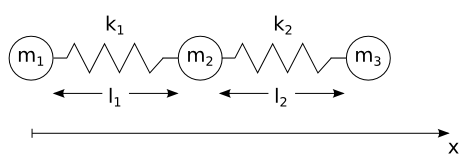
\includegraphics[width=0.8\textwidth]{images/3-masses-2-springs-linear.png}
\caption{Diagram for 3 masses attached with springs representing the nuclei motion.}
\label{fig:3-masses-2-springs}
\end{figure}

Consider 3 masses $m_i,\ i=1,2,3$ attached linearly by two springs of constants $k_1$ and $k_2$ and rest length of $l_1$ and $l_2$ respectively (later we will let $ m_1=m_3$, $ k_1=k_2$ and $l_1=l_2$). 
We will look only at the motion in the longitudinal direction so we attach a reference frame and call $ x_i$ ($i=1,2,3$) the coordinate describing the position of $m_i$.
A lagrangian $L$ for this system is 

\begin{align}
L & = T-V\\
  & = \frac{1}{2}\sum_{i=1}^3 m_i \dot{x}_i^2 - \frac{1}{2}k_1(l_1-(x_2-x_1))^2+\frac{1}{2}k_2(l_2-(x_3-x_2))^2
\end{align}

It will be more convenient to change the $x_i$ coordinates to another set reflecting only the displacements from the equilibrium position.
That is, we define new coordinates $\eta_i$ such that $(x_1,x_2,x_3)=(\eta_1,l_1+\eta_2,l_1+l_2+\eta_3)$. 
In this coordinate system the lagrangian looks simpler

\begin{equation}
  L= \frac{1}{2}\sum_{i=1}^3 m_i \dot{\eta}_i^2-\frac{1}{2}k_1(\eta_1-\eta_2)^2+\frac{1}{2}k_2(\eta_2-\eta_3)^2
\end{equation}

The potential energy is a quadratic function of the $\eta_i$ displacements so we can write it in the general form $V=\frac{1}{2}\sum_{i,j}V_{ij}\eta_i\eta_j$ where $V_{ij}$ are the elements of the matrix defined as

\begin{equation}
  (V_{ij})=\left( \begin{array}{ccc} k_1 & -k_1 & 0 \\ -k_1 & k_1+k_2 & -k_2 \\ 0 & -k_2 & k_2 \end{array} \right)
\end{equation}

The dynamics of the system is determined by the Euler-Lagrange equations,

\begin{align}
  0 & = \frac{d}{dt}\frac{\partial L}{\partial \dot{\eta}_s}-\frac{\partial L}{\partial \eta_s} \label{eq:EulLag1} \\
    & = m_s \ddot{\eta}_s + \sum_i V_{is} \eta_i \label{eq:EulLag2}
\end{align}

\noindent for $s=1,2,3$. 
We can propose an oscillatory solution of the form $\eta_i=a_ie^{i\omega t}$, understanding that only the real part of this equations describe the real motion of the cluster. 
Substituting this solution into the equations of motion (\ref{eq:EulLag2}), after removing the common exponential factor, gives

\begin{equation}
  0=\sum_i V_{is}a_i-\omega^2m_sa_s
\end{equation}

which can be arranged as a matrix

\begin{equation}
  \left( 
    \begin{array}{c} 
      0\\ 0\\ 0 
    \end{array}
  \right) = (V_{ij}) \left(
    \begin{array}{c}
      a_1 \\ a_2 \\ a_3 
    \end{array}
  \right) - \omega^2 \left(
    \begin{array}{ccc}
      m_1 & 0 & 0 \\ 0 & m_2 & 0 \\ 0 & 0 & m_3
    \end{array}\right) \left(
    \begin{array}{c} 
      a_1 \\ a_2 \\ a_3 
    \end{array}
  \right)
\end{equation}

Substituting the actual values for $(V_{ij})$:

\begin{equation}
  \left( 
    \begin{array}{c}
      0\\ 0\\ 0
    \end{array}
  \right) 
  = \left(
    \begin{array}{ccc}
      k_1-\omega^2m_1 & -k_1 & 0 \\ -k_1 & k_1+k_2-\omega^2m_2 & -k_2 \\ 0 & -k_2 & k_2-\omega^2m_3 
    \end{array}
  \right) 
  \left(
    \begin{array}{c}
      a_1 \\ a_2 \\ a_3 
    \end{array}
  \right)
\end{equation}

In order to have a non-trivial solution we require the determinant of that matrix to be zero

\begin{equation}
  \label{eq:det}
  \begin{split}
    0 = & (k_1-\omega^2m_1)(k_1+k_2-\omega^2m_2)(k_2-\omega^2m_3) \\
        & -k_1^2(k_2-\omega^2m_3)-k_2^2(k_1-\omega^2m_1)
  \end{split}
\end{equation}

\noindent which is a third order alebraic equation for $\omega^2$ with 3 solutions for $\omega$.
To simplify the calculation we take now into consideration the details of our problem, that is, we consider $m_1 = m_3 \equiv m_O$, $m_2 \equiv m_{Cu}$ and $k_1 = k_2 \equiv k$. 
With this considerations, (\ref{eq:det}) simplifies to

\begin{align}
  \label{eq:omegas}
  0 & = (k-\omega^2m_O)^2(2k-\omega^2m_{Cu})-2k^2(k-\omega^2m_O) \\
    & = (k-\omega^2m_O)[(k-\omega^2m_O)(2k-\omega^2m_{Cu})-2k^2]
\end{align}

\noindent from which we can observe one solution

\begin{equation}
  \omega^2= \frac{k}{m_O}
\end{equation}

\noindent corresponding to the symmetrical (Raman) vibrational mode, denoted by $\omega_{R}$ in \ref{eq:phonon-part}, since it doesn't depend on $m_{Cu}$.
The other two frequencies are obtained from the remaining factor in \ref{eq:omegas},

\begin{equation}
  \begin{split}
    0 & = (k-\omega^2m_O)(2k-\omega^2m_{Cu})-2k^2 \\
      & = 2k^2-k\omega^2m_{Cu}-2k\omega^2m_O+\omega^4m_Om_{Cu}-2k^2 \\
      & = \omega^2[\omega^2m_Om_{Cu}-k(m_{Cu}+2m_O)]
  \end{split}
\end{equation}

\noindent from here we obtain the uninteresting $\omega^2=0$ and

\begin{equation}
  \omega^2 = \frac{k(m_{Cu}+2m_O)}{m_Om_{Cu}}
\end{equation}

This is the frequency of the asymmetric (infrared) vibrational mode, denoted by $\omega_{ir}$ in (\ref{eq:phonon-part}).
Summarizing this part, we have found the dependency of the phonon frequencies $\omega_{ir}$ and $\omega_R$ with the atomic masses for the oxygen $m_O$ and copper $m_{Cu}$ atoms in the following way

\begin{equation}
  \label{eq:omegaR}
  \omega_{R}= \sqrt{\frac{k}{m_O}}
\end{equation}

\begin{equation}
  \label{eq:omegair}
  \omega_{ir} = \sqrt{\frac{k(m_{Cu}+2m_O)}{m_Om_{Cu}}}
\end{equation}

\noindent for some constant $k$.
Also, from here we identify the reduced masses for each vibrational mode

\begin{equation}
  \label{eq:redMassR}
  m_R \equiv m_O \simeq 16.0\ u \simeq 2.6568 \times 10^{-26} kg
\end{equation}

\begin{equation}
  \label{eq:redMassIr}
  m_{ir} \equiv \frac{m_Om_{Cu}}{m_{Cu}+2m_O} \simeq 10.64\ u \simeq 1.7668 \times 10^{-26}kg
\end{equation}

\subsection{Change in the coupling constants}

Also, the coupling parameters depend on $m_O$\cite{?}:

\begin{equation}
  \label{eq:ir-coupl-isot}
  \lambda_{ir}\propto (m_O\omega_{ir})^{-1/2}
\end{equation}

\begin{equation}
  \label{eq:Ram-coupl-isot}
  \lambda_R\propto (m_O\omega_{R})^{-1/2}
\end{equation}


\subsection{Effects of changing the oxygen mass}

From the discussion in the previous sections, it can be seen that an oxygen isotpe substitution, $^{16}$O $\rightarrow$ $^{18}$O ammounts to a change in the frequencies  $(\omega_{ir}$, $\omega_R)$ and the coupling constants $(\lambda_{ir},\lambda_R)$.
We now turn to the task of finding the ammount of such changes.
Denoting as $\omega^{(16)}$ and $\omega^{(18)}$ the phonon frequencies for a cluster with $^{16}$O and $^{18}$O respectively, from (\ref{eq:omegair}, \ref{eq:omegaR}) we can calculate the ratios

\begin{align}
  \omega^{(16)}_{ir}/\omega^{(18)}_{ir}
  & =\sqrt{\left(\frac{m_{^{18}O}}{m_{^{16}O}}\right)\left(\frac{m_{Cu}+2m_{^{16}O}}{m_{Cu}+2m_{^{18}O}}\right)} \\
  \omega^{(16)}_{R}/\omega^{(18)}_{R}
  & =\sqrt{\frac{m_{^{18}O}}{m_{^{16}O}}}
\end{align}

Taking the actual values for copper and oxygen, $m_{Cu}=63.546u$, $m_{^{16}O}=15.995u$ and $m_{^{18}O}=17.999u$, we obtain

\begin{equation}
  \label{eq:omega-ir-isot}
  \omega^{(16)}_{ir} / \omega^{(18)}_{ir} \simeq 1.039
\end{equation}

\begin{equation}
  \label{eq:omega-R-isot}
  \omega^{(16)}_{R} / \omega^{(18)}_{R} \simeq 1.061
\end{equation}

Similarly, for the coupling constants $\lambda_{ir}$ and $\lambda_R$, from (\ref{eq:ir-coupl-isot}, \ref{eq:Ram-coupl-isot}) we can observe that

\begin{equation}
  \label{eq:lambda-ir-isot}
  \lambda_{ir}^{(16)}/\lambda_{ir}^{(18)}=\sqrt{\frac{m_{^{18}O}\omega_{ir}^{(18)}}{m_{^{16}O}\omega_{ir}^{(16)}}}\simeq 1.0407
\end{equation}

\noindent and similarly for the Raman coupling constant

\begin{equation}
  \label{eq:lambda-Ram-isot}
  \lambda_R^{(16)} / \lambda_R^{(18)} \sqrt{\frac{m_{^{18}O}\omega_{R}^{(18)}}{m_{^{16}O}\omega_{R}^{(16)}}} \simeq 1.0299
\end{equation}

Summarizing, to model an isotopic substitution $^{16}$O$\rightarrow ^{18}$O we need to adjust the vibrational frequencies and coupling constants according to equations (\ref{eq:omega-ir-isot}-\ref{eq:lambda-Ram-isot})

\subsection{Definition of isotopic shifts}

% Motivation missing

We define the relative isotopic shift for an excited state $i$ as 

\begin{equation}
  \label{eq:isot-shift-def-exc}
  \Delta_i = \frac{E_i(^{16}O)- E_i(^{18}O)}{E_i(^{16}O)} \times 100
\end{equation}

\noindent where the energies $E_i$ are referred to the corresponding ground state.

For the ground state we define the energy isotopic shift $\Delta_g$ in a similar way but with the energies measured relative to the uncoupled system, that is, the system with $\lambda_{ir}=\lambda_R=0$,

\begin{equation}
  \label{eq:isot-shift-def-grd}
  \Delta_g = \frac{\Delta E_g(^{16}O)- \Delta E_g(^{18}O)}{\Delta E_g(^{16}O)} \times 100
\end{equation}

\noindent where $\Delta E_g \equiv E_g - E_g(\lambda_{ir}=0, \lambda_R=0)$.

\section{Lattice distortions}
\label{sec:lattice-distortions}

To understand the lattice distortion for excitations in the model hamiltonian (\ref{eq:full-hamiltonian}) it is useful to find the projection of a given state to real space atomic coordinates. 
In a simple quantum harmonic oscillator with mass $m$ and frequency $\omega$ the creation and annihilation operators, $a^\dagger$ and $a$, are related to the real-space coordinate $x$ as

\begin{equation}
  \label{eq:harmOscRel}
  x=\sqrt{\frac{\hbar}{2m\omega}}\left(a+a^\dagger\right)
\end{equation}

If we assume that phonon modes in our model hamiltonian (\ref{eq:phonon-part}) behave as quantum harmonic oscillators, we can define symmilar real space operators ($u_r,u_{ir}$) in terms of the bosonic creation and annihilation operatos ($b^\dagger,b$) for both, infrared and Raman, vibrational modes. 
These operators, called \textit{phonon coordinates}, are also related to the positions $x_i$ of the three sites in the cluster \cite{MustredeLeon1992},

\begin{equation}
  \label{eq:uR}
  u_R \equiv \left(\frac{\hbar}{2 m_R \omega_R}\right)^{1/2}(b_R^\dagger + b_R) = \frac{x_3 - x_1}{\sqrt{2}}
\end{equation}

\begin{equation}
  \label{eq:uir}
  u_{ir} \equiv \left(\frac{\hbar}{2 m_{ir} \omega_{ir}}\right)^{1/2}(b^\dagger_{ir}+b_{ir}) = \frac{ x_1 + x_3 - ( 2 m_O/m_{Cu})x_2}{(2 + 4 m_O/m_{Cu})^{1/2}}
\end{equation}

The reduced masses $m_R$ and $m_{ir}$ are determined in equations (\ref{eq:redMassR}, \ref{eq:redMassIr}).
In a quantum harmonic oscillator an energy eigenfunction, $\ket{n}$, has a projection into the real space coordinate $x$ given in terms of a Hermite polynomial $H_n(x)$ of degree $n$ in the following way,

\begin{equation}
  \label{eq:harmOscProj}
  \braket{x}{n} 
  \equiv \psi_n(x) 
  = \frac{1}{\sqrt{2^n n!}} \left(\frac{m \omega}{\pi \hbar}\right)^{1/4}
  \exp\left(-\frac{m \omega x^2}{2 \hbar}\right) H_n\left( \sqrt{\frac{m \omega}{\hbar}} x \right) 
\end{equation}


For an arbitrary wavefunction $\ket{\psi} = \sum_n \braket{n}{\psi} \ket{n}$ the projection in real space is $\braket{x}{\psi} = \sum_n \braket{n}{\psi} \braket{x}{n}$ with $\braket{x}{n}$ given by \ref{eq:harmOscProj}.

For the model hamiltonian (\ref{eq:full-hamiltonian}), as discussed in section \ref{sec:hamiltonian-and-basis}, a possible basis set is given by the functions ${| e_1, e_2, ir, R \rangle}$ with $e_i$ the position of the $i$-th electron and $ir$, $R$ the number of infrared and Raman phonons respectively. 
Thus an arbitrary wavefunction in this system, $\ket{\psi}$, can be expanded as

\begin{equation}
  \label{eq:wf-phonon-base}
  \ket{\psi}=\sum_{e_1,e_2,ir,R} \braket{e_1,e_2,ir,R}{\psi}\ket{e_1,e_2,ir,R}
\end{equation}

\noindent and we can make the partial projection into the phonon coordinates $(u_{ir},u_R)$ as defined by (\ref{eq:uR},\ref{eq:uir})

\begin{equation}
  \label{eq:wf-expansion}
  \braket{u_{ir},u_R}{\psi}=\sum_{e_1,e_2,ir,R} \braket{e_1,e_2,ir,R}{\psi}\braket{u_{ir},u_R}{ir,R}\ket{e_1,e_2}
\end{equation}

\noindent where we have denoted $\braket{u_{ir},u_r}{e_1,e_2,ir,R}=\braket{u_{ir},u_R}{ir,R}\ket{e_1,e_2}$. 
The term $\braket{u_{ir},u_r}{ir,R}$ is similar to (\ref{eq:harmOscProj}) but considering both phonon modes:

\begin{equation}
  \label{eq:hermite-expansion}
  \braket{u_{ir},u_r}{ir,R}  = \frac{\left(m_{ir}m_R\right)^{1/4}}{\sqrt{2^{(ir+R)} ir!R!\pi\hbar}}
  \exp\left(-\frac{\tilde{u}_{ir}^2 + \tilde{u}_R^2}{2}\right) 
  H_{ir}\left(\tilde{u}_{ir} \right)H_{R}\left(\tilde{u}_{R} \right)
\end{equation}

\noindent where we have defined the normalized coordinates,

\begin{equation}
  \label{eq:uTildeDef}
  \tilde{u}_j \equiv \sqrt{\frac{m_j\omega_x}{\hbar}}\ u_j
\end{equation}

\noindent for $j=ir,R$. 
Now, from (\ref{eq:wf-expansion}), the probability amplitude of findind a state $\ket{\psi}$ proyected into phonon coordinates $(u_{ir},u_R)$ for a given site occupation $(e_1,e_2)$ is

\begin{equation}
  \begin{split}
    & \left|\braket{e_1,e_2,u_{ir},u_R}{\psi}\right|^2 \\
    & \ \ = \left|\sum_{e_1',e_2',ir,R}\braket{e_1,e_2,ir,R}{\psi}\braket{u_{ir},u_R}{ir,R}\braket{e_1,e_2}{e_1',e_2'}\right|^2 \\
    & \ \ = \left|\sum_{ir,R}\braket{e_1,e_2,ir,R}{\psi}\braket{u_{ir},u_R}{ir,R}\right|^2
  \end{split}
\end{equation}

Finally, the probability amplitude of finding a system in the state $\ket\psi$ with phonon coordinates ($u_{ir},u_R$) irrespective of the electronic configuration is given by the sum over the electronic degrees of freedom on the previous equation,

\begin{equation}
  \label{eq:phonon-coord-projection}
  \begin{split}
    \left|\psi(u_{ir}, u_R)\right|^2 & \equiv \sum_{e_1,e_2}\left|\braket{e_1,e_2,u_{ir},u_R}{\psi}\right|^2 \\
    & = \sum_{e_1,e_2} \left|\sum_{ir,R}\braket{e_1,e_2,ir,R}{\psi}\braket{u_{ir},u_R}{ir,R}\right|^2
  \end{split}
\end{equation}

\noindent with $\braket{u_{ir},u_R}{ir,R}$ given by (\ref{eq:hermite-expansion}).

The projection \ref{eq:phonon-coord-projection} allows us to calculate the probability amplitude of finding a specific distortion in the atomic coordinates for the O-Cu-O cluster.
With the atomic coordinates $x_i$, as defined in section \ref{sec:isotopic-model}, the difference $d$ in O-Cu bond lengths is

\begin{equation}
  \label{eq:bondDiff}
  d= \left| (x_3 - x_2) - (x_2 - x_1) \right| = \left| x_1 + x_3 - 2x_2 \right|
\end{equation}

The $x_i$ coordinates are varying at all times but taking an instant in which $x_2=0$ we can simplify (\ref{eq:bondDiff}) to

\begin{equation}
  \label{eq:bondDiffSimpl}
  d=\left|x_1+x_3\right|
\end{equation}

From $u_{ir}$'s definition in (\ref{eq:uir}),

\begin{equation}
  \label{eq:uirSimpl}
  u_{ir}=\frac{x_1+x_3}{\left( 2+4 m_O/m_{Cu} \right)^{1/2}}
\end{equation}

Now, using (\ref{eq:bondDiffSimpl}) and (\ref{eq:uirSimpl}), we find that

\begin{equation}
  \label{eq:uirvsd}
  \left|u_{ir}\right|=\frac{d}{\left( 2+4 m_O/m_{Cu} \right)^{1/2}}
\end{equation}

\noindent or, solving for $d$,

\begin{equation}
  \label{eq:dvsuir}
  d=\sqrt{2}\left(1 + 2\frac{m_O}{m_{Cu}} \right)^{1/2}\left|u_{ir}\right|
\end{equation}

\noindent which is a relationship between the phonon coordinates, that can be calculated from the model's eigenfunctions, and the observable lattice distortion. 
Equation (\ref{eq:dvsuir}) allows a conection between this model hamiltonian and a specific experimental observation. 
It is this relationship that helps fixing the variable coupling parameters $\lambda_{ir}$ and $\lambda_R$.

\section{Projection into states with definite electron occupation numbers}
\label{sec:electronic-projection}

Eigenstates of the hamltonian \ref{eq:full-hamiltonian}, in general, have delocalized charges.
To understand charge dynamics according for each excitation it is useful to project the eigenstates into the definite electron occupation basis states discussed in section \ref{sec:hamiltonian-and-basis}.
The basis set we are using ($\{\ket{e_1,e_2,ir,R}\}$) has sharp values for the hole number operator on each site for a given number of infrared $ir$ and Raman $R$ phonons. 
Thus, to find the probability $P(e_1,e_2)$ of finding one hole in site $e_1$ and the other on site $e_2$, we need only to sum over the infrared and Raman phonons of the system,

\begin{equation}
  \label{eq:electron-occupation}
  P(e_1,e_2)=\sum_{ir,R} \left| \braket{e_1,e_2,ir,R}{\psi} \right|^2
\end{equation}

From the labeling convention stated in (\ref{eq:label}) we can visualize the nine possible combinations of hole occupancy. 
Denoting, for example, $e_1$ as $\uparrow$ and $e_2$ as $\downarrow$ we have the following combinations:

\begin{equation}\label{eq:basis-set}
\begin{array}{cccc}
1= & \uparrow \downarrow & - & - \\
2= & \uparrow & \downarrow & - \\
3= & \uparrow & - & \downarrow \\
4= & \downarrow & \uparrow & - \\
5= & - & \uparrow \downarrow & - \\
6= & - & \uparrow & \downarrow \\
7= & \downarrow & - & \uparrow \\
8= & - & \downarrow & \uparrow \\
9= & - & - & \uparrow \downarrow 
\end{array}
\end{equation}

Since the model hamiltonian (\ref{eq:full-hamiltonian}) does not distinguish spin and the cluster is symmetrical, states (1, 9) are equivalent, as well as (2, 4, 6, 8) and (3, 7).

\section{Choice of parameters}
\label{sec:model-parameters}

To choose values for this model we take representative values guided from local-density approximations \cite{Pickett1989}. 
In particular Ref. \cite{DeWeert1989}, using a tight-binding model, reports a band energy of $E_0$ = 0.35 eV and a hopping parameter of $t=0.43-0.74$ eV, for Cu(1)-O(4) sites.
The on-site Coulomb repulsion in La$_2$CuO$_4$, $U$  is estimated to be in the range $4.0-10.5$ eV, \cite{Hybertsen1989}. 

The bare phonon frequencies are fixed to values found experimentally in optical and inelastic neutron scattering experiments $\omega_R = 500$ cm$^{-1}$ and $\omega_{ir} = 612.4$ cm$^{-1}$ for YBa$_2$Cu$_3$O$_7$ \cite{?}.

In order to consider the simplest possible model we make the further assumption of taking the on-site Coulomb repulsion in the copper and oxygen sites to be equal with no nearest neighbor Coulomb repulsion. 
We also use a single hopping parameter $t$ and ignore hopping between the two oxygen sites. 
Since only the coupling between the asymmetric mode and the charge motion leads to a measurable lattice distortion, with two Cu–O bond lengths, we only consider the effect of the variation in the electron–lattice coupling constant with the antisymmetric mode, $\lambda_{ir}$, and we set the electron-lattice coupling with the symmetric mode, $\lambda_R$ , as zero \cite{Salkola1995}. 
The inclusion of those considerations in the model, or other choices of parameters (e.g. \cite{Salkola1994, Salkola1995}) yield very similar results.
The relevant value for the coupling $\lambda_{ir}$ is determined using equation \ref{eq:dvsuir}; it is chosen such that the ground state has a maximum probability density at a $u_{ir}$ that reproduces the observed lattice distortion of 0.13 \AA \cite{?}.
In this work we use the same parameters as \cite{DeLeon1999, Leon2008, MirandaMena2007,Mena2006}, namely:

\begin{itemize*}
\item On-site Coulomb repulsion for O(4) and Cu(1) sites: $U=7$ eV
\item Nearest-neighbor hopping: $t=0.5$ eV
\item Band energy for O(4) and Cu(1) sites: $E_0=0.5$ eV
\item Bare phonon frequency for the Raman mode: $\omega_R=500$ cm$^{-1}$
\item Bare phonon frequency for the infrared mode: $\omega_{ir}=612.4$ cm$^{-1}$
\end{itemize*}

As previously stated, some variation in the parameter space has been explored without changes in the basic phenomenology. Table \ref{tab:parameters} shows the parameters for this model used in other publications\footnote{It seems that the reported values for the phonon frequencies in \cite{Salkola1994, Salkola1995} are erroneous since they show $\omega_R > \omega_{ir}$ and they are inconsistent from what can be observed in Fig. 1 of \cite{Salkola1994} at $\lambda_{ir}=0$.}.

\begin{table}[h]
  \centering
  \begin{tabular}[h]{| l | c | c | c | c | c |}
    \hline
    Reference & $U$ (eV) & $\epsilon$ (eV) & $t$ (eV) & $\omega_{ir}$ (cm$^{-1}$) & $\omega_R$(cm$^{-1)}$ \\
    \hline
    \cite{MustredeLeon1992} & 7.0 & 0.5 & 0.5 & 600 & 500 \\ 
    \cite{Salkola1994, Salkola1995} & 4.44 & 0.307 & 0.634 & 477.7 & 576  \\
    \cite{DeLeon1999, Leon2008, MirandaMena2007,Mena2006} & 7.0 & 0.5 & 0.5 & 612.4 & 500 \\ 
    \cite{MustredeLeon2000} & 4.44 & 0.307 & 0.634 & 600 & 500 \\
    \hline
  \end{tabular}
  \caption{Parameters for the model hamiltonian (\ref{eq:full-hamiltonian}) used in other publications.}
  \label{tab:parameters}
\end{table}

\section{Classification of the excitations}
\label{sec:classification}

As previously noted in section \ref{sec:hamiltonian-and-basis}, only for zero electron-lattice couplings the eigenstates of the many-body Hamiltonian (\ref{eq:full-hamiltonian}) can be described as a direct product of purely electronic and phononic states. 
In this scenario each eigenstate has a sharp value for the phonon number operators $b_Rb^\dagger_R$ and $b_{ir}b^\dagger_{ir}$ allowing its identification as a \textit{phononic} state with a given number of phonons, an \textit{electronic} state or a simple product of those two.
However, for electron-lattice couplings larger than zero, the phonon number operator has some dispersion and the eigenstates are no longer purely \textit{phononic} or \textit{electronic} in nature.
It is this mixing of electronic and lattice states that allows the exact treatment used in this work to explore a phenomenology not reachable with the adiabatic and anti-adiabatic approximations.

% - Following the eigenvalue, mean ir (Ram) and their dispersions we can track them with increasing couling (plot?)
% Maybe include the plot projecting the electronic state at \lambda_{ir}>0 with itself at \lambda_{ir}=0


\section{Computational details}
\label{sec:comp_details}

We performed an exact diagonalization of the Hamiltonian matrix with a basis of 8649 states using a QR algorithm \cite{eigenweb}\footnote{The hamiltonian (\ref{eq:full-hamiltonian}) is a sparse matrix, so a more efficient approach is being taken in subsequent calculations, in extensions of this model, using Lanczos algorithm. In this work we used a QR algorithm because it was readily available and provided a large enough basis set to ensure convergence.}.
The basis includes up to 30 harmonic Raman and 30 harmonic infrared phonons. 
The  truncation of the basis to a finite number of phonons could introduce innacuracies, however we found this choice to be an adecuate choice to ensure convergence in the few lowest energy states we are considering and electron-lattice couplings up to $\sim0.25$ eV\footnote{There is another numerical instability present in the calculation of the isotopic shift of the first excitation (see section \ref{sec:polaron-isotopic-shift}) but this seems to be due to floating point errors in the calculations since all numbers are very close to zero.}.

% Maybe a plot here showing convergence in the energy of the ground state for different number of phonons?